%%%%%%%%%%%%%%%%%%%%%%%%%%%%%%%%%%%%%%%%%%%%%%%%%
\newpage
%%%%%%%%%%%%%%%%%%%%%%%%%%%%%%%%%%%%%%%%%%%%%%%%%

\subsection{weitere Diagramme}


\begin{figure}[hptb]
 \centering
 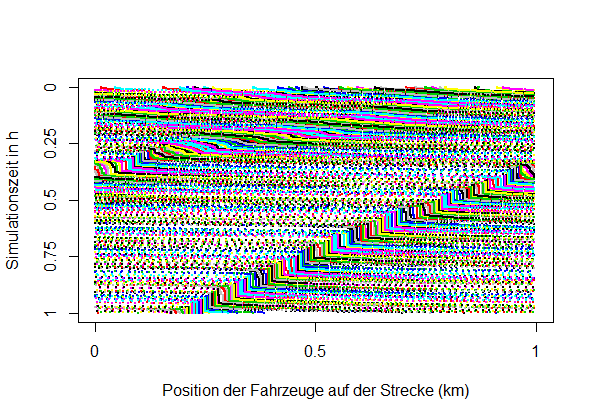
\includegraphics[width=1\textwidth]{33veh-1km}
 \caption{Positionsdiagramm mit rückwärts laufender Stauwelle}
 \label{figure:33veh-1km}
\end{figure}

\cref{figure:33veh-1km} entstand aufgrund einer Fehleinstellung in der Szenariodatei.
Hier fuhren 33 Fahrzeuge auf einer Strecke von 1 km.
Für diese kurze Strecke ist diese Anzahl Fahrzeuge nicht zu bewältigen.
\\
Zu Beginn sieht man aufgrund der enger werdenden Punktmuster, dass sich die Geschwindigkeit der Fahrzeuge nur verlangsamt. Dann kommt es zu einer länger anhaltenden Stillstandsphase der Fahrzeuge, die auch zu Simulationsende noch anhielt.
\\
Hier erkennt man die in den Versuchen in \cite{na-sch} erkannte Rückwärtsbewegung der Stauwelle.


%%%%%%%%%%%%%%%%%%%%%%%%%%%%%%%%%%%%%%%%%%%%%%%%%
\newpage
%%%%%%%%%%%%%%%%%%%%%%%%%%%%%%%%%%%%%%%%%%%%%%%%%


\begin{figure}[hptb]
  \centering
   \subfigure[34 Fzg]{\includegraphics[width=1\textwidth]{a7-34veh-position-2nd}\label{figure:a7-34veh-position-2nd}} \\
   \subfigure[34 Ftg]{\includegraphics[width=1\textwidth]{a7-34veh-position-noflow}\label{figure:a7-34veh-position-noflow}}
  \caption{weitere Simulationsläufe mit 34 Fahrzeugen, A7-Verkehrsmenge}
  \label{figure:a7-34veh-more}
\end{figure}

Positionsplots weiterer Simulationsläufe mit der A7-Verkehrsmenge (siehe \cref{sec:szenario-a7}) zeigen, dass auch mit 34 Fahrzeugen Stockungen auftreten können.
Oft passierte dies zu Beginn des Durchlaufes, pendelte sich dann aber ein.


%%%%%%%%%%%%%%%%%%%%%%%%%%%%%%%%%%%%%%%%%%%%%%%%%
\newpage
%%%%%%%%%%%%%%%%%%%%%%%%%%%%%%%%%%%%%%%%%%%%%%%%%


\begin{figure}[hptb]
  \centering
   \subfigure[mit 36 Fahrzeugen]{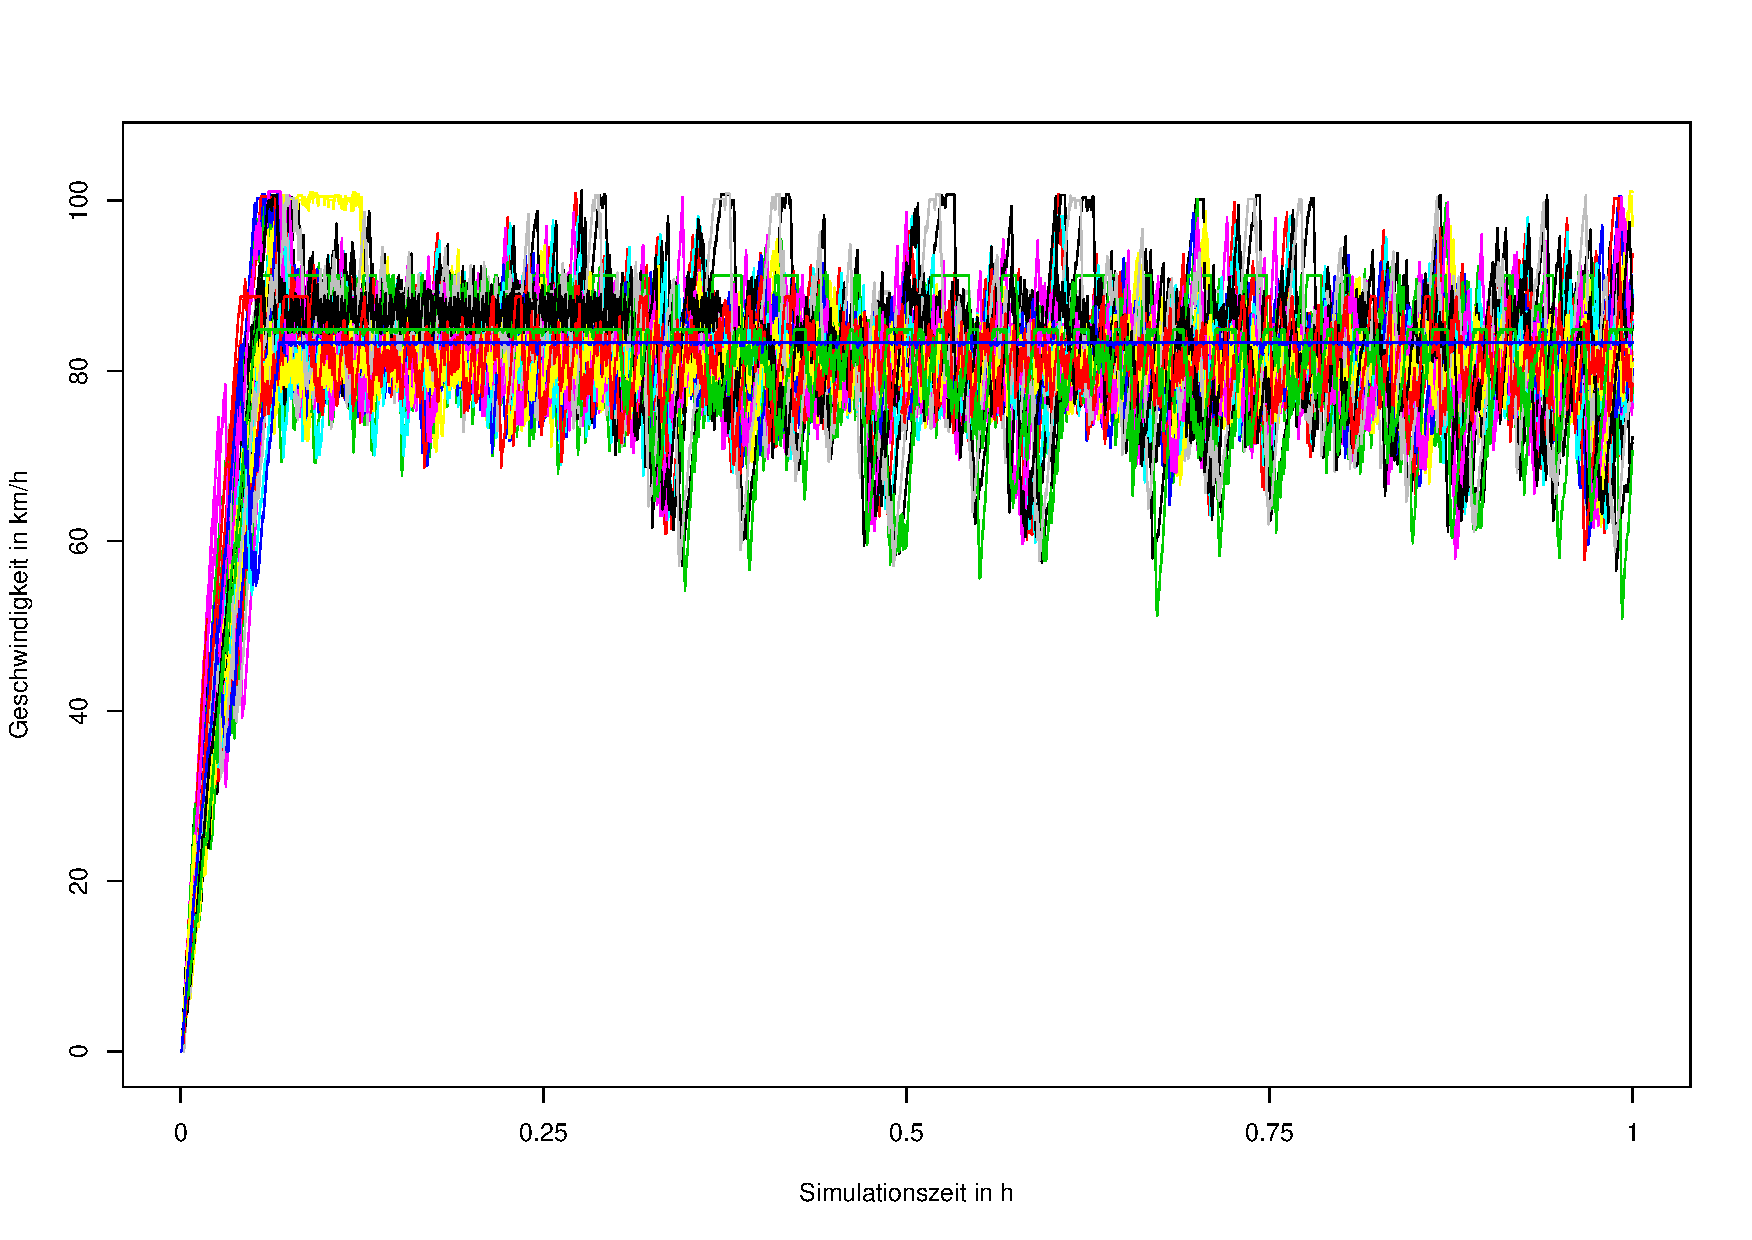
\includegraphics[width=0.3\textwidth]{short-a7-36-speed}\label{figure:short-a7-36-speed}}\qquad 
   \subfigure[mit 37 Fahrzeugen]{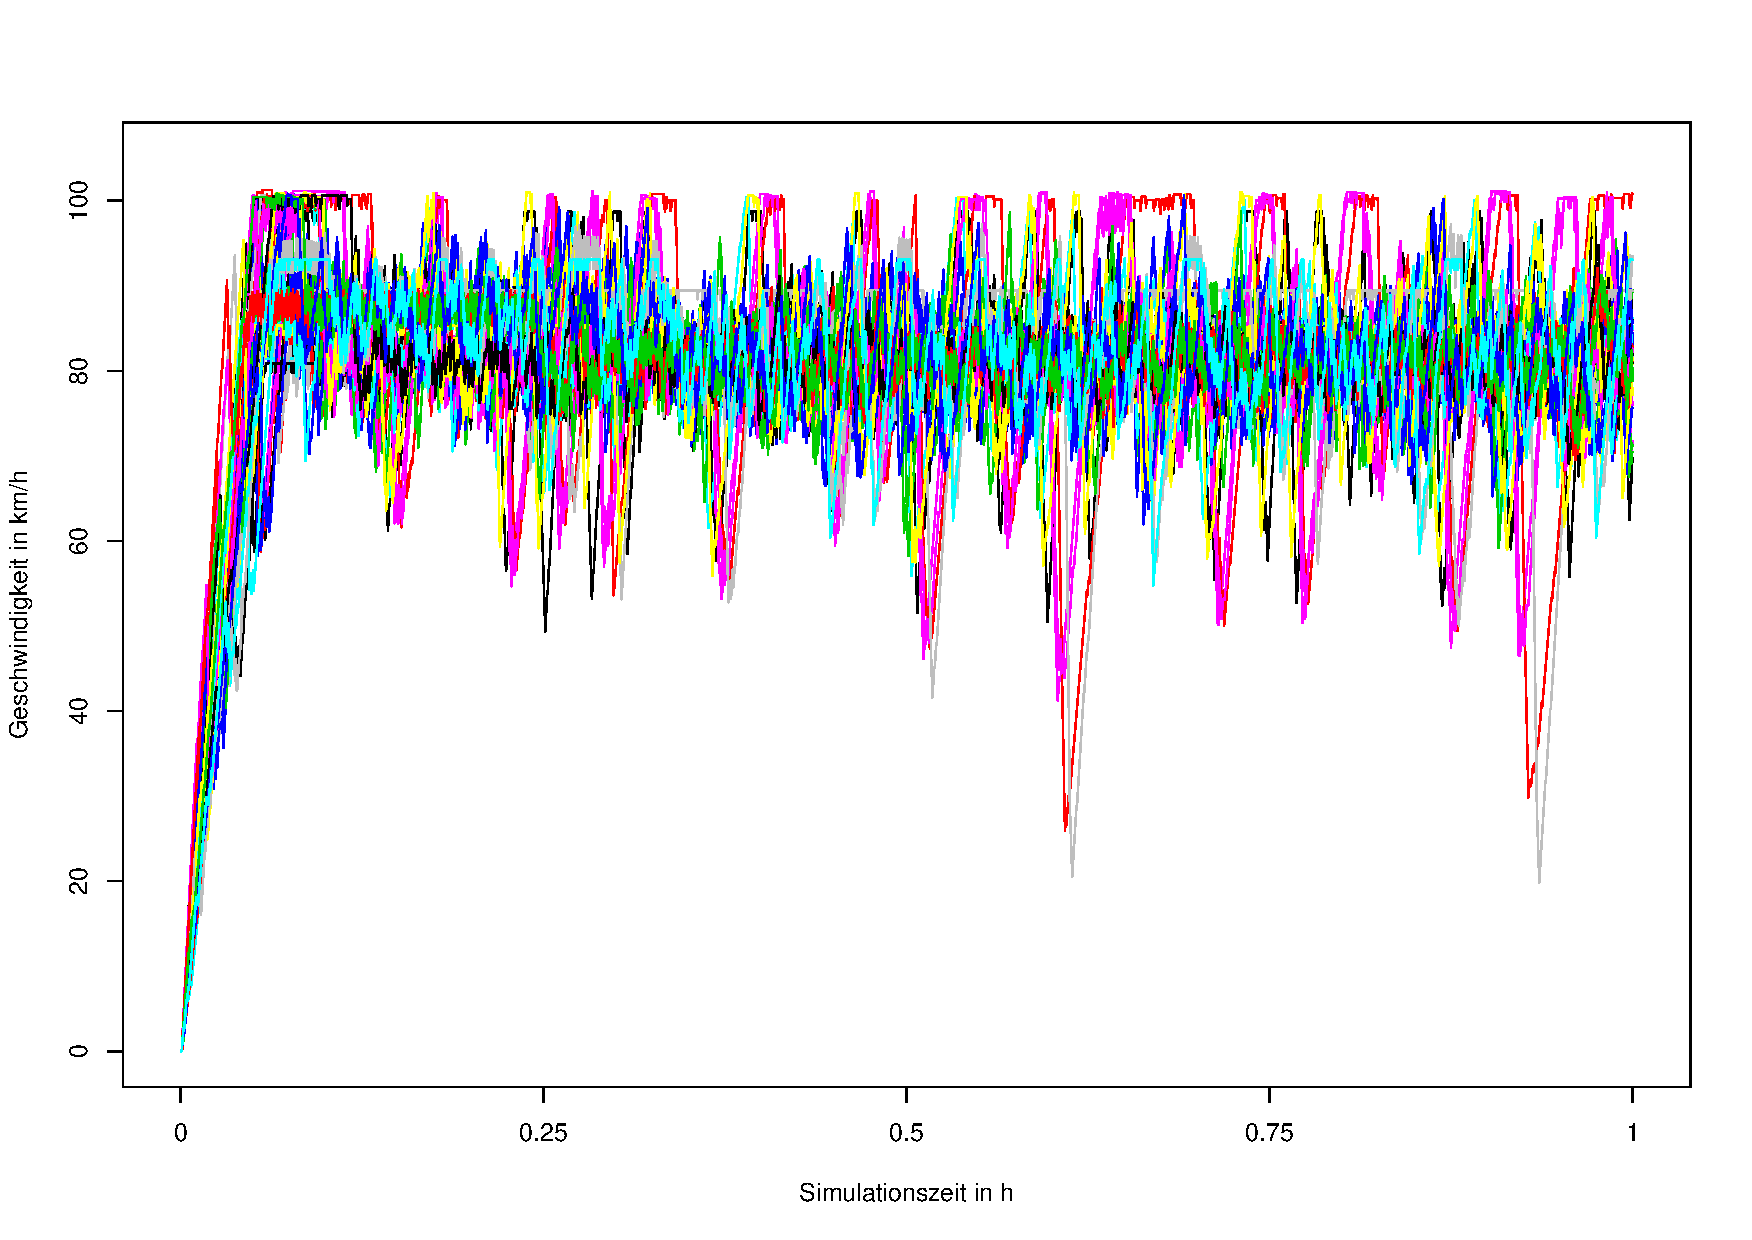
\includegraphics[width=0.3\textwidth]{short-a7-37-speed}\label{figure:short-a7-37-speed}}\qquad 
   \subfigure[mit 38 Fahrzeugen]{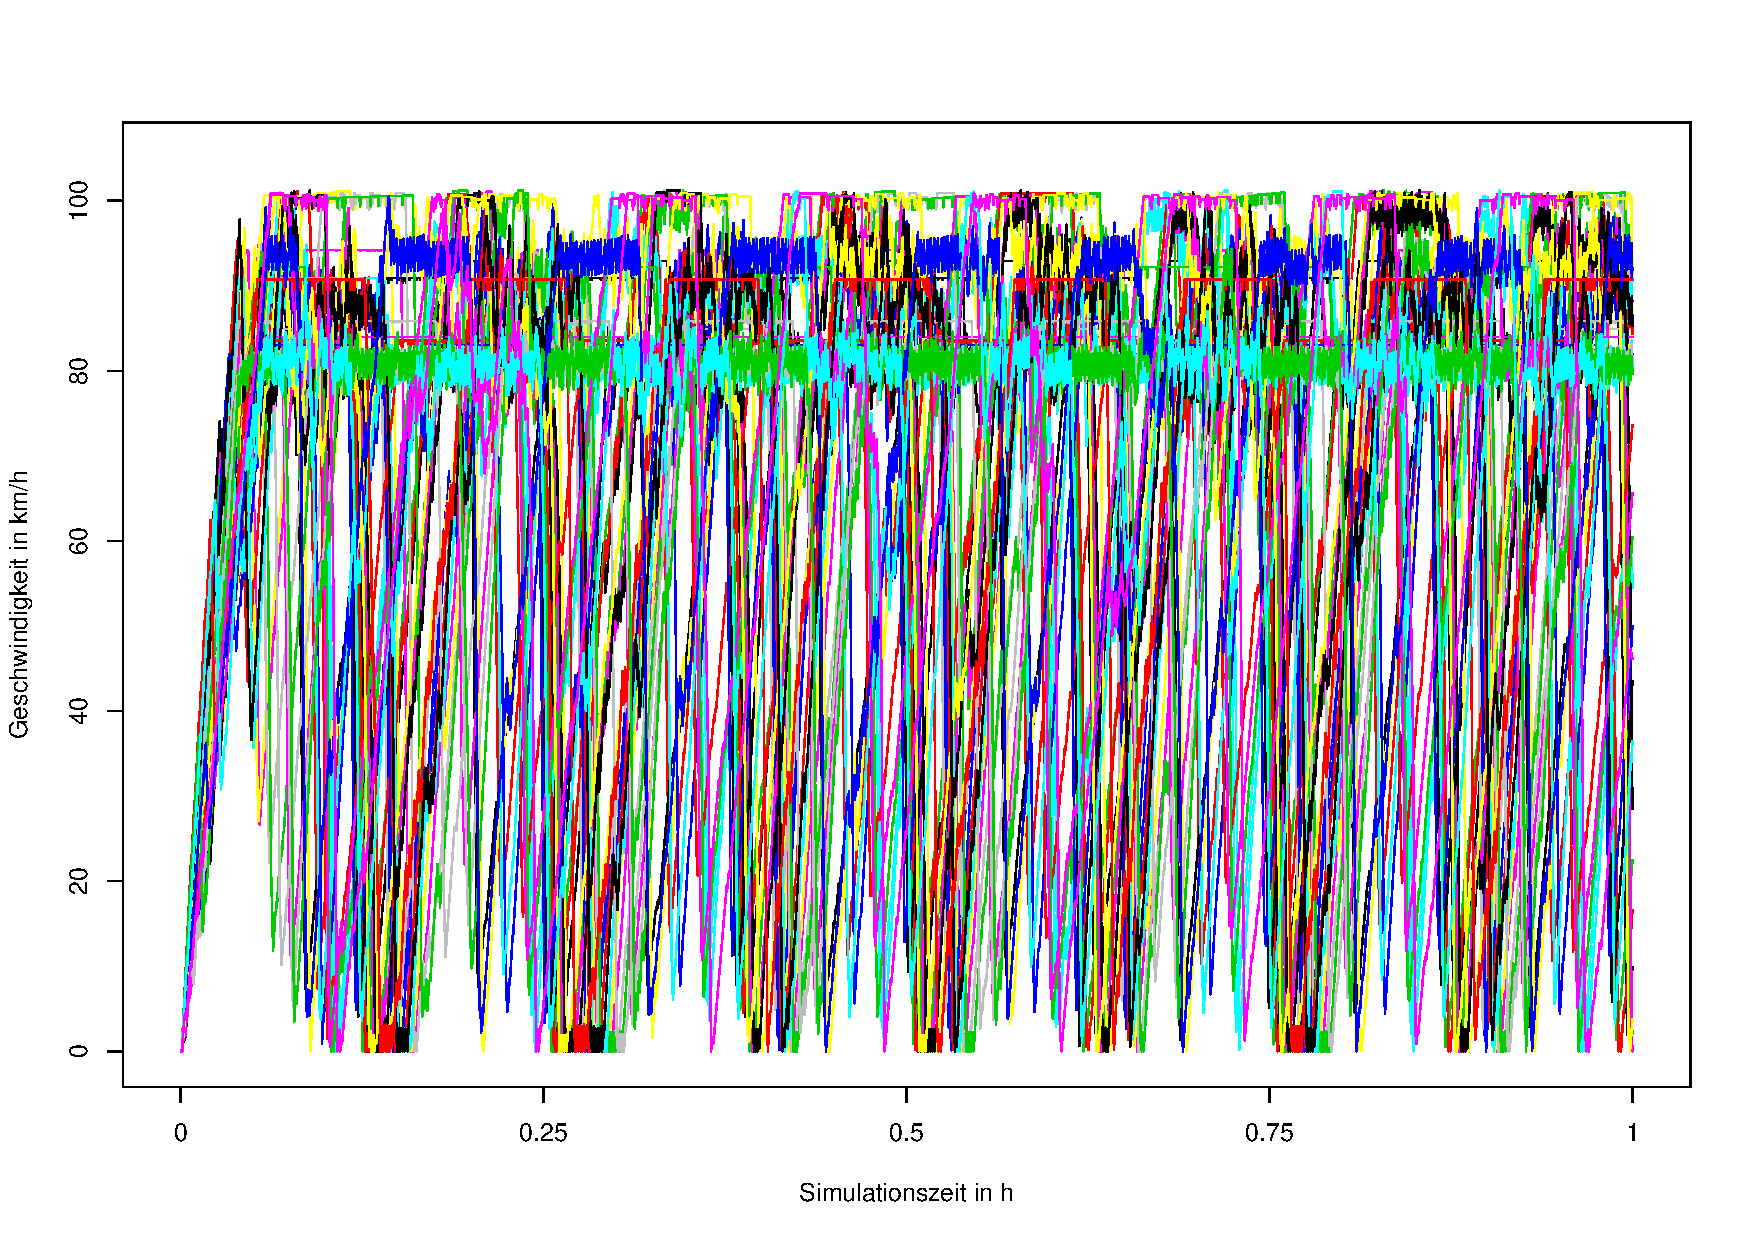
\includegraphics[width=0.3\textwidth]{short-a7-38-speed}\label{figure:short-a7-38-speed}} \\
   \subfigure[mit 38 Fahrzeugen (Positionen)]{\includegraphics[width=1\textwidth]{short-a7-38-position}\label{figure:short-a7-38-position}}
  \caption{Geschwindigkeitskurven der erweiterten Testläufe}
  \label{figure:short-a7}
\end{figure}

\cref{figure:short-a7} zeigt drei Geschwindigkeitskurven und ein Positionsplot für die Simulationsläufe der fahrzeugweisen Erhöhung der Verkehrsmenge der A7 aus \cref{sec:szenario-a7}.

Bereits ab einer Menge von 37 Fahrzeugen sind die Einbrüche der Geschwindigkeitskurven wesentlich stärker ausgeprägt (\cref{figure:short-a7-37-speed}).
Der Verkehrsfluss kann aber noch aufrecht erhalten werden.

Mit 38 Fahrzeugen und mehr kommt es dann zu mehreren kleineren Stauereignissen.
Während sich die Ereignisse auf der Fahrbahn vorwärts bewegen, ist in jeweils die Rückwärtsbewegung der Stauwelle erkennbar (\cref{figure:short-a7-38-position}).


%%%%%%%%%%%%%%%%%%%%%%%%%%%%%%%%%%%%%%%%%%%%%%%%%
\newpage
%%%%%%%%%%%%%%%%%%%%%%%%%%%%%%%%%%%%%%%%%%%%%%%%%


\begin{figure}[hptb]
  \centering
   \subfigure[Position]{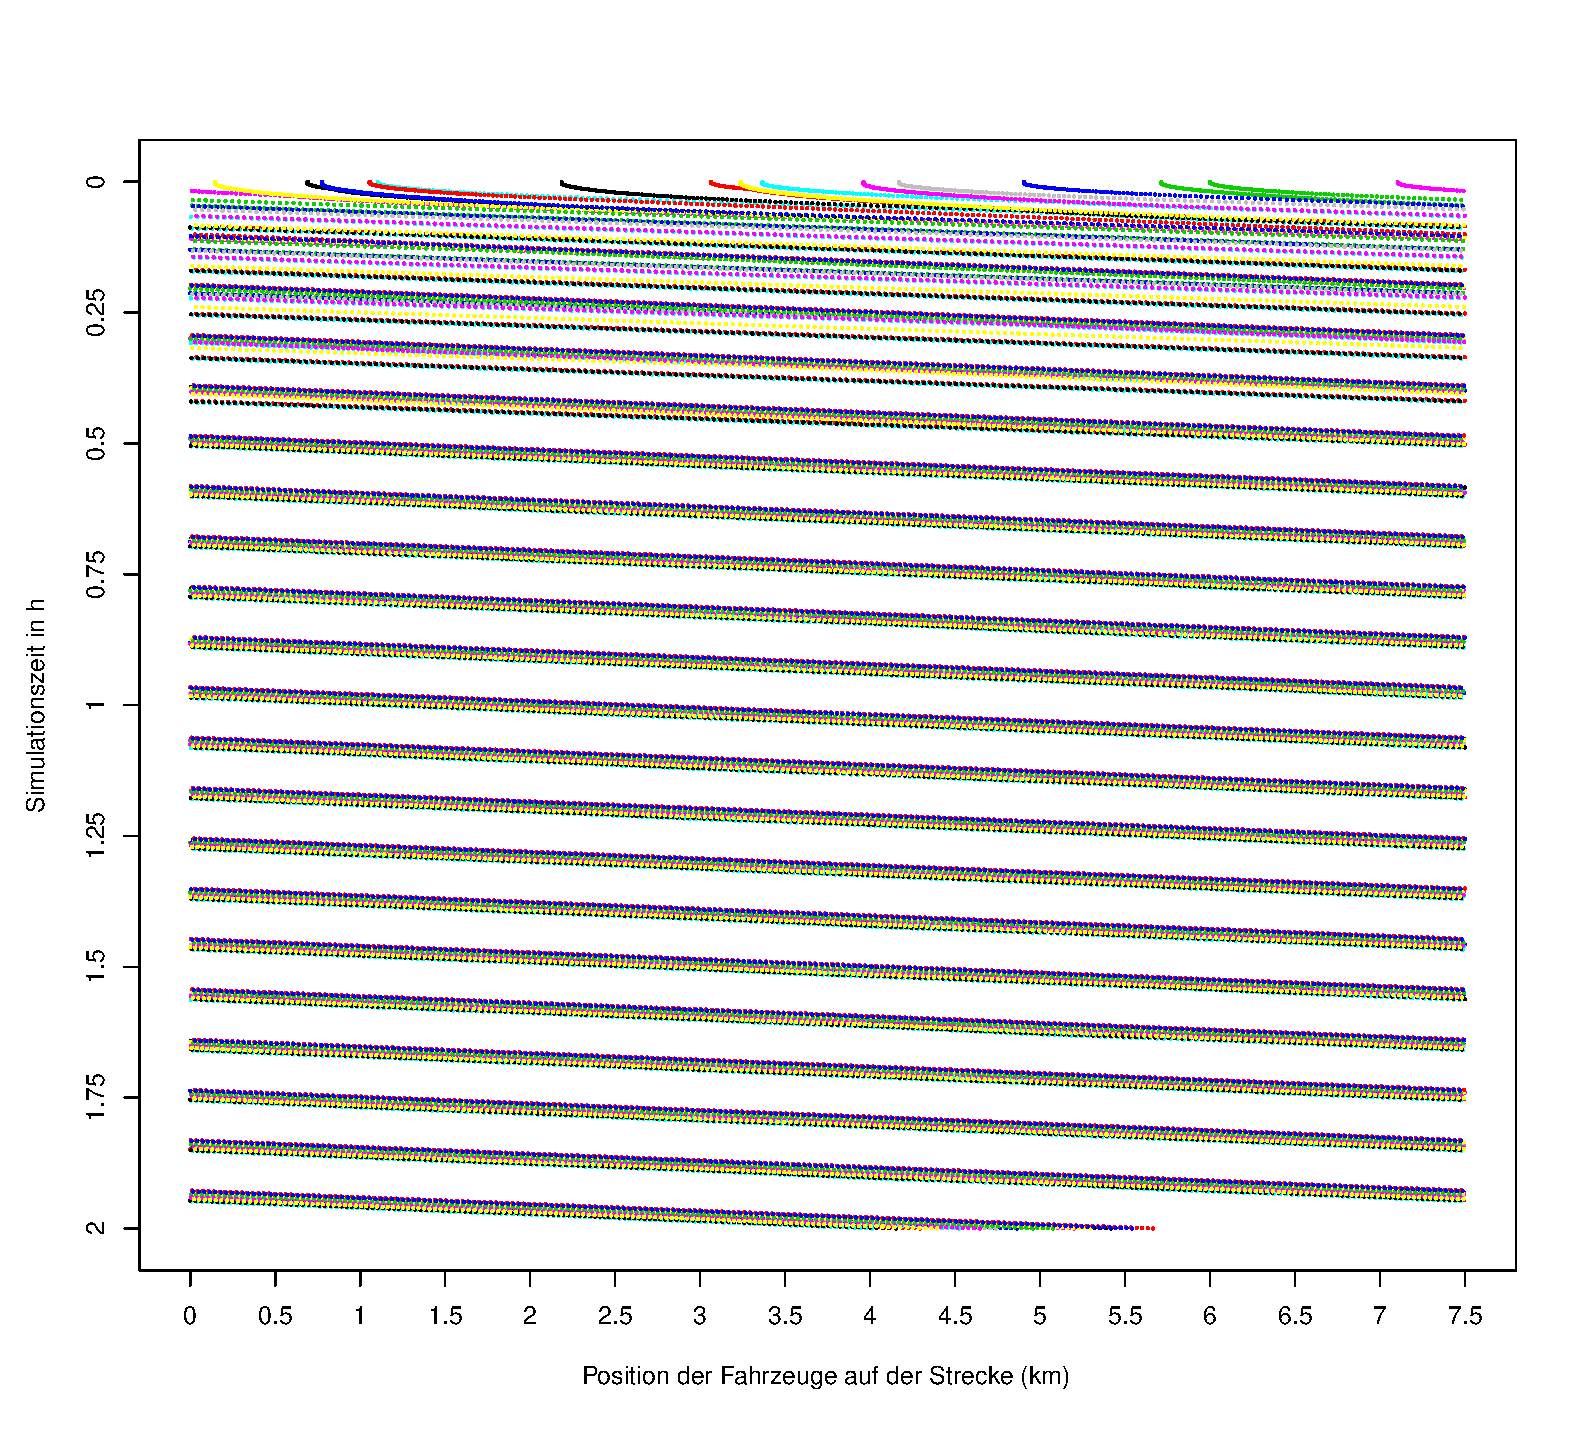
\includegraphics[width=1\textwidth]{a38-position}\label{figure:a38-position}} \\
   \subfigure[Geschwindigkeit]{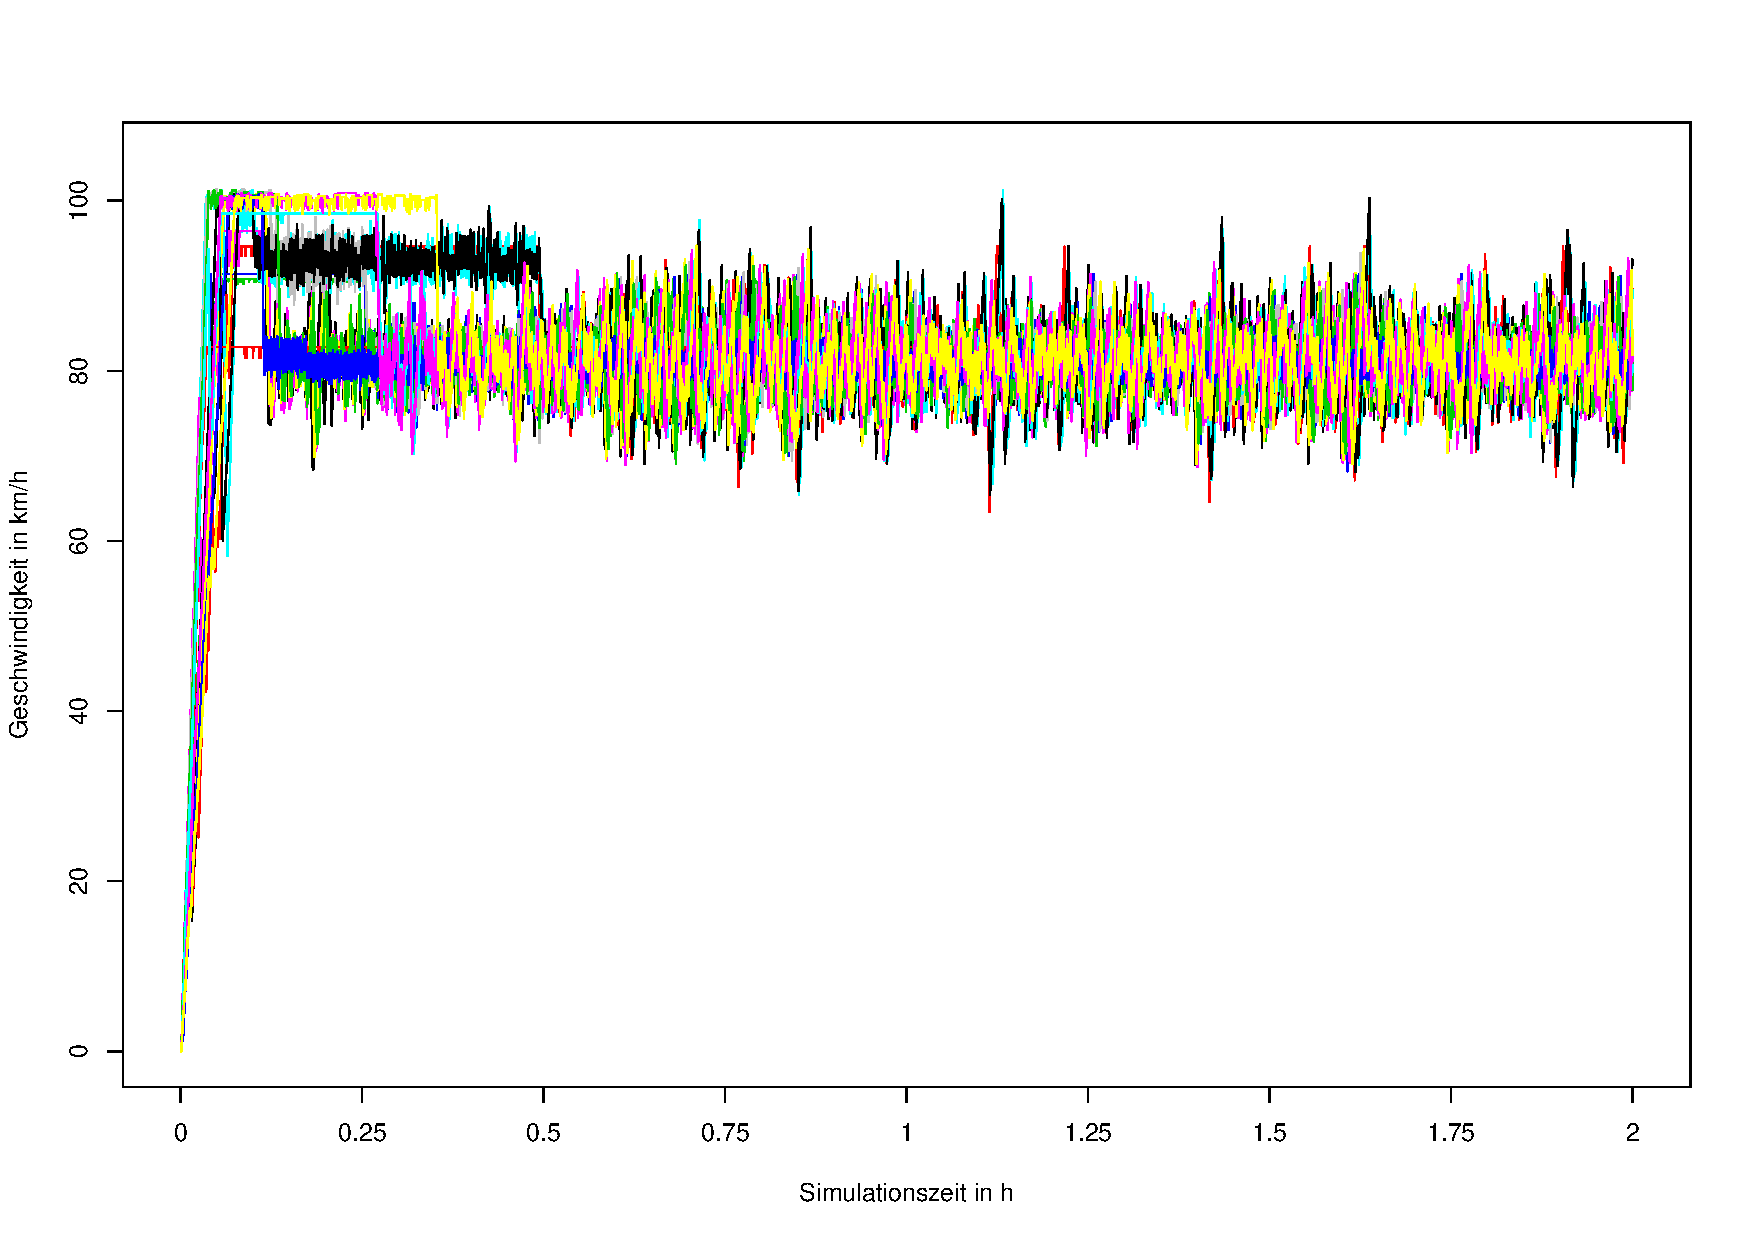
\includegraphics[width=1\textwidth]{a38-speed}\label{figure:a38-speed}}
  \caption{Diagramme, A38-Verkehrsmenge: 15 Fahrzeuge}
  \label{figure:a38-position-speed}
\end{figure}

\sa{own: content}


%%%%%%%%%%%%%%%%%%%%%%%%%%%%%%%%%%%%%%%%%%%%%%%%%
\newpage
%%%%%%%%%%%%%%%%%%%%%%%%%%%%%%%%%%%%%%%%%%%%%%%%%


\begin{figure}[hptb]
  \centering
   \subfigure[Position]{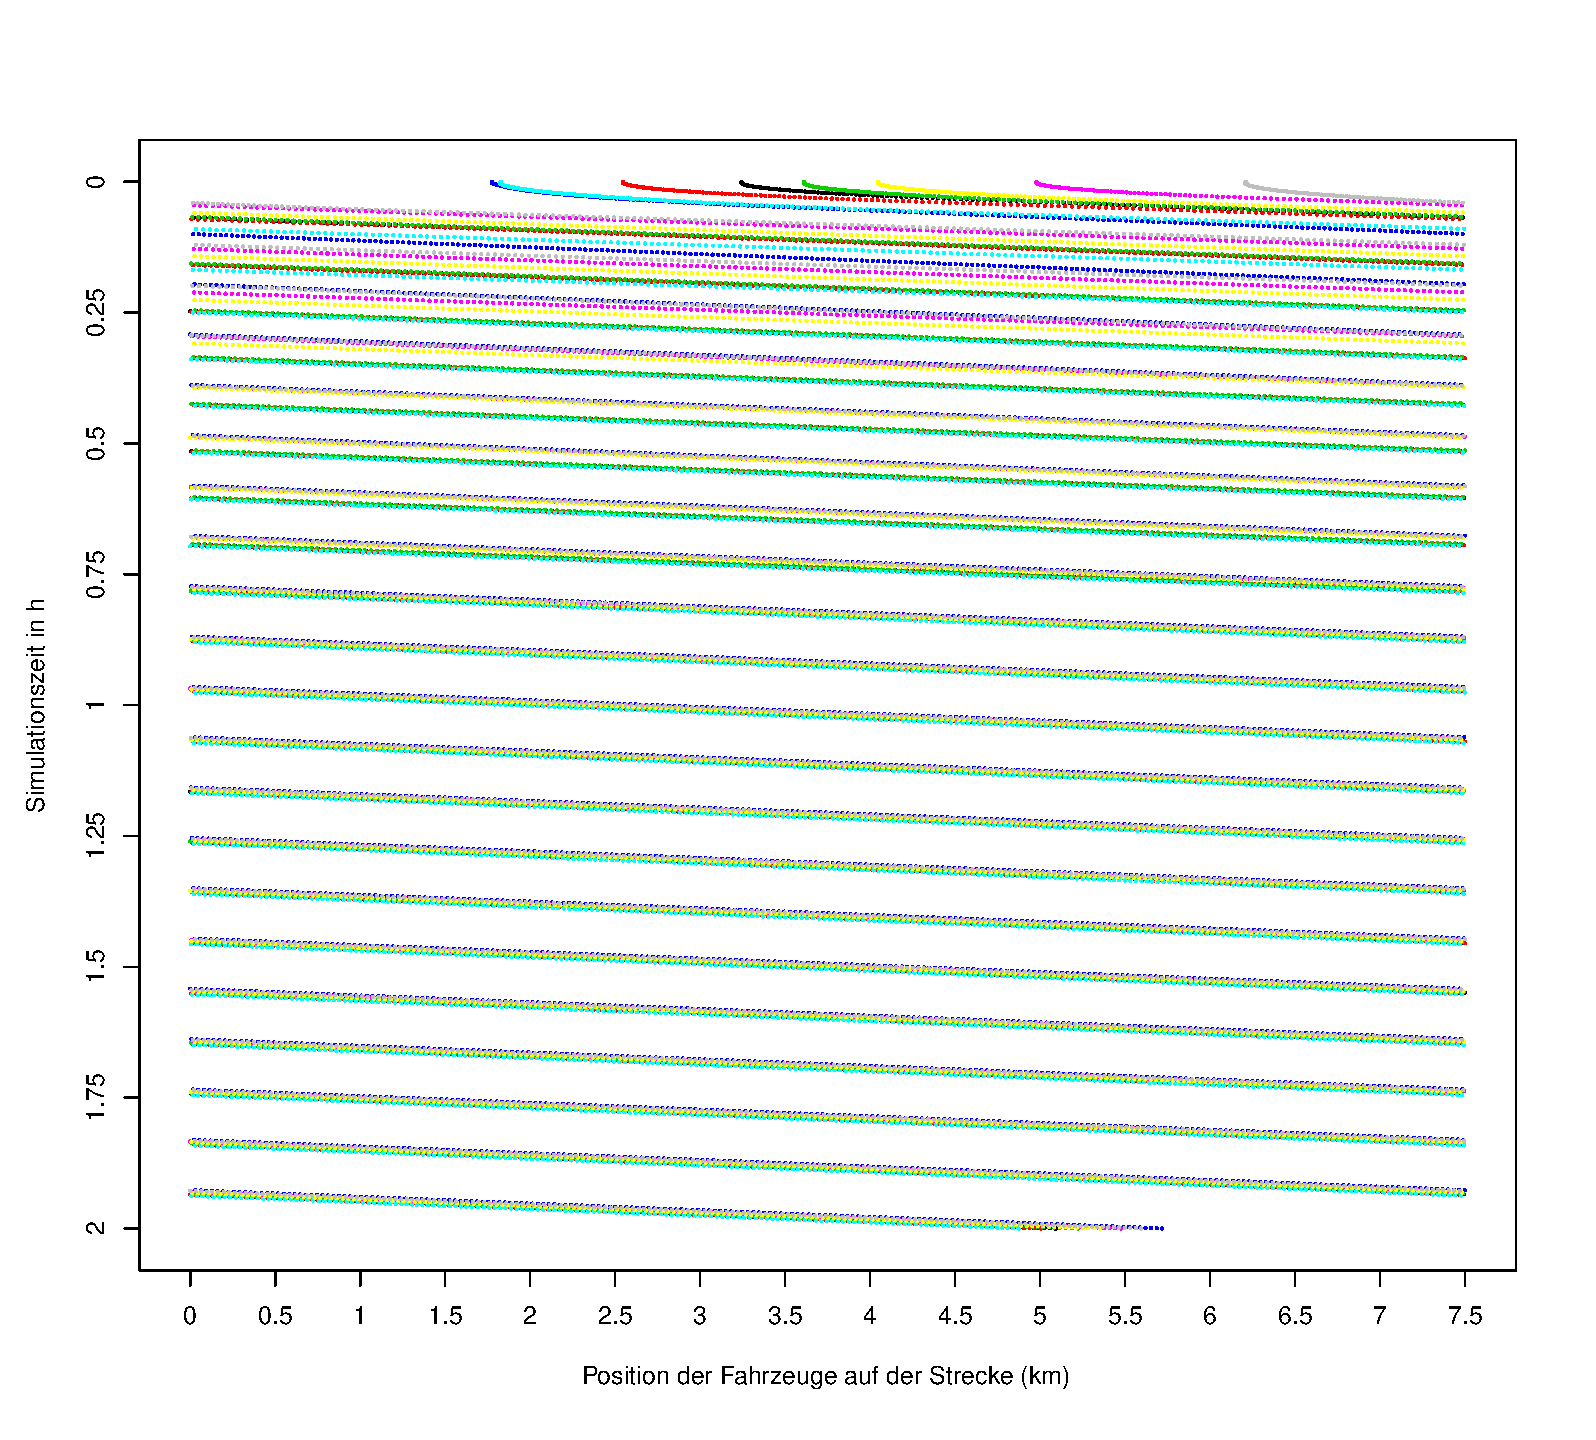
\includegraphics[width=1\textwidth]{a71-position}\label{figure:a71-position}} \\
   \subfigure[Geschwindigkeit]{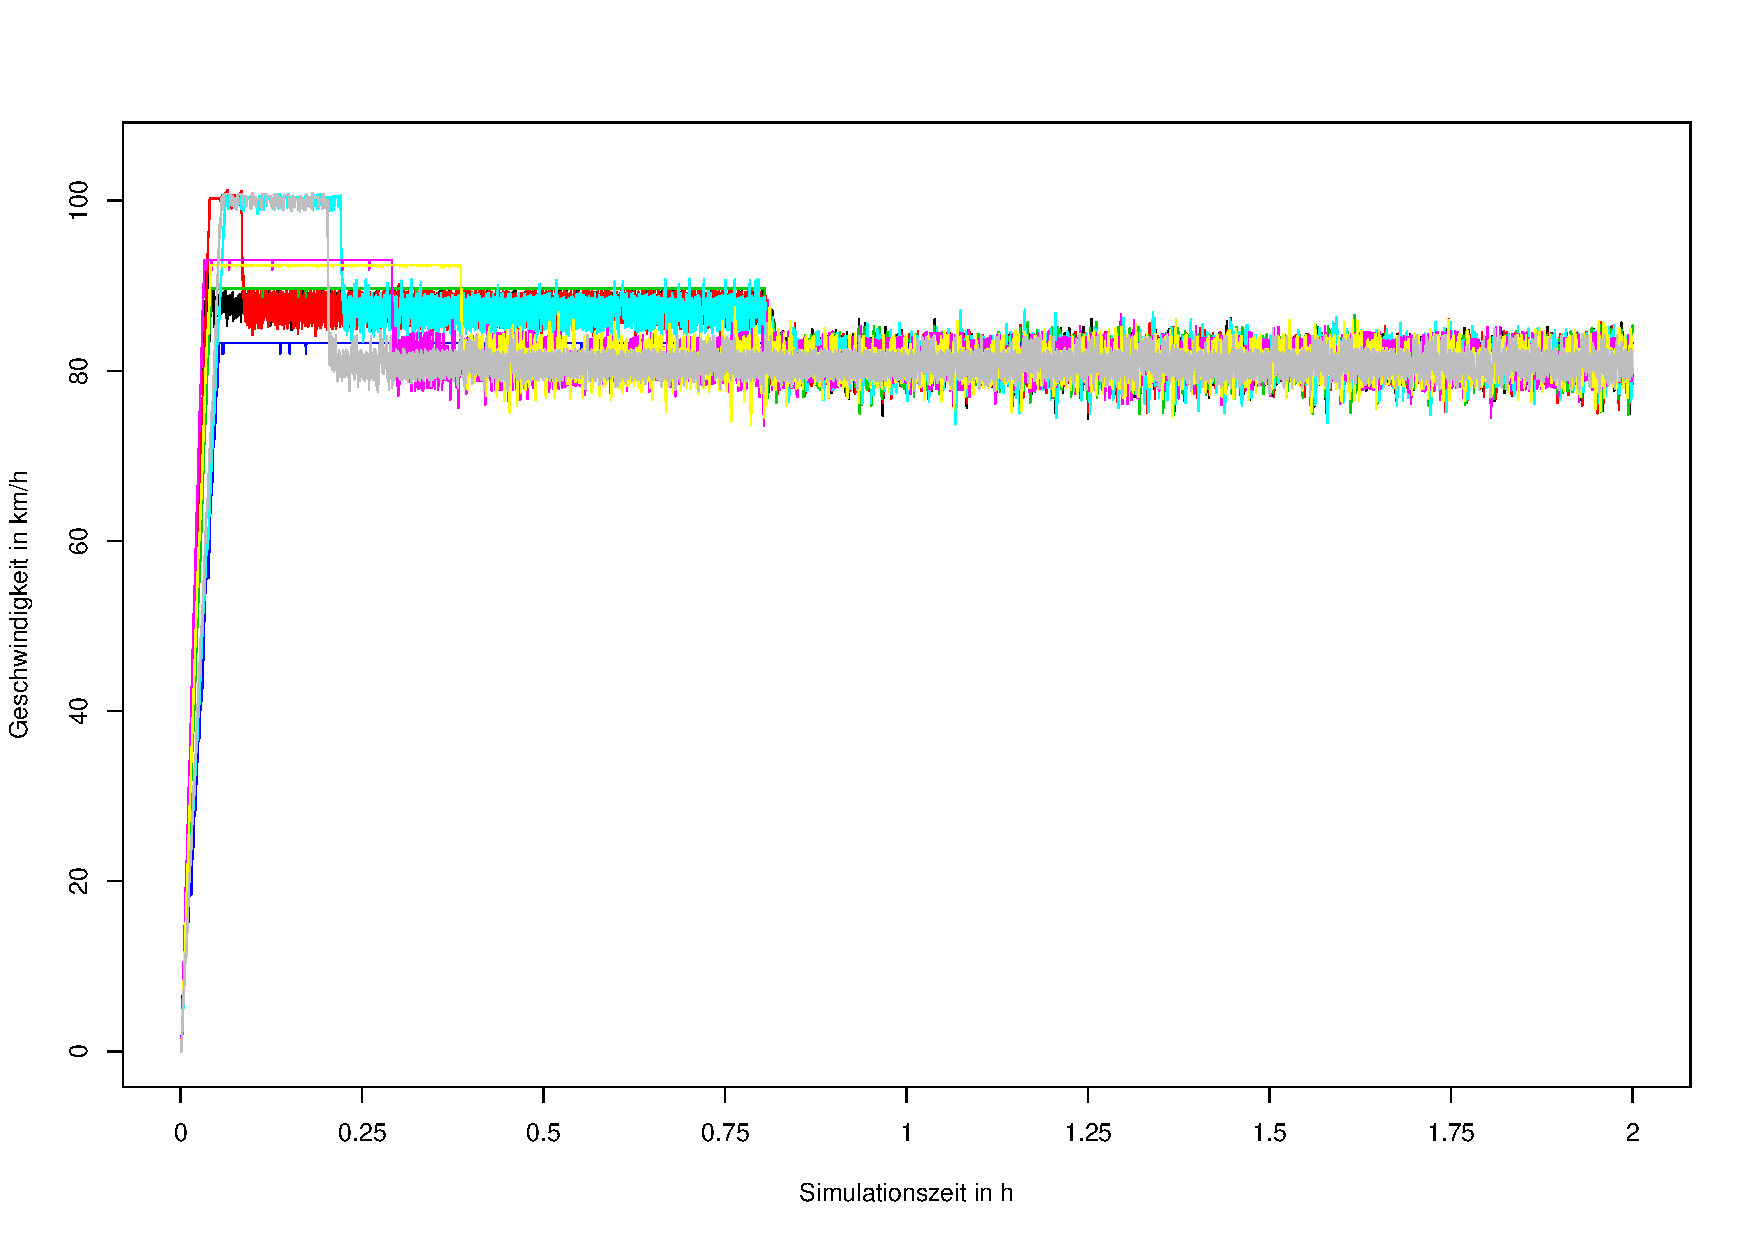
\includegraphics[width=1\textwidth]{a71-speed}\label{figure:a71-speed}}
  \caption{Diagramme, A71-Verkehrsmenge: 8 Fahrzeuge}
  \label{figure:a71-position-speed}
\end{figure}

\sa{own: content}




%%%%%%%%%%%%%%%%%%%%%%%%%%%%%%%%%%%%%%%%%%%%%%%%%

	%   %	%   %	 %%%%	%%%%%	%%%%%	%%%%
	%% %%	%   %	%		  %		%		%   %
	% % %	%   %	 %%%	  %		%%%		%%%%
	%   %	%   %	    %	  %		%		%  %
	%   %	 %%%	%%%%	  %		%%%%%	%	%

%%%%%%%%%%%%%%%%%%%%%%%%%%%%%%%%%%%%%%%%%%%%%%%%%
%
%\begin{figure}[hptb]
% \centering
% 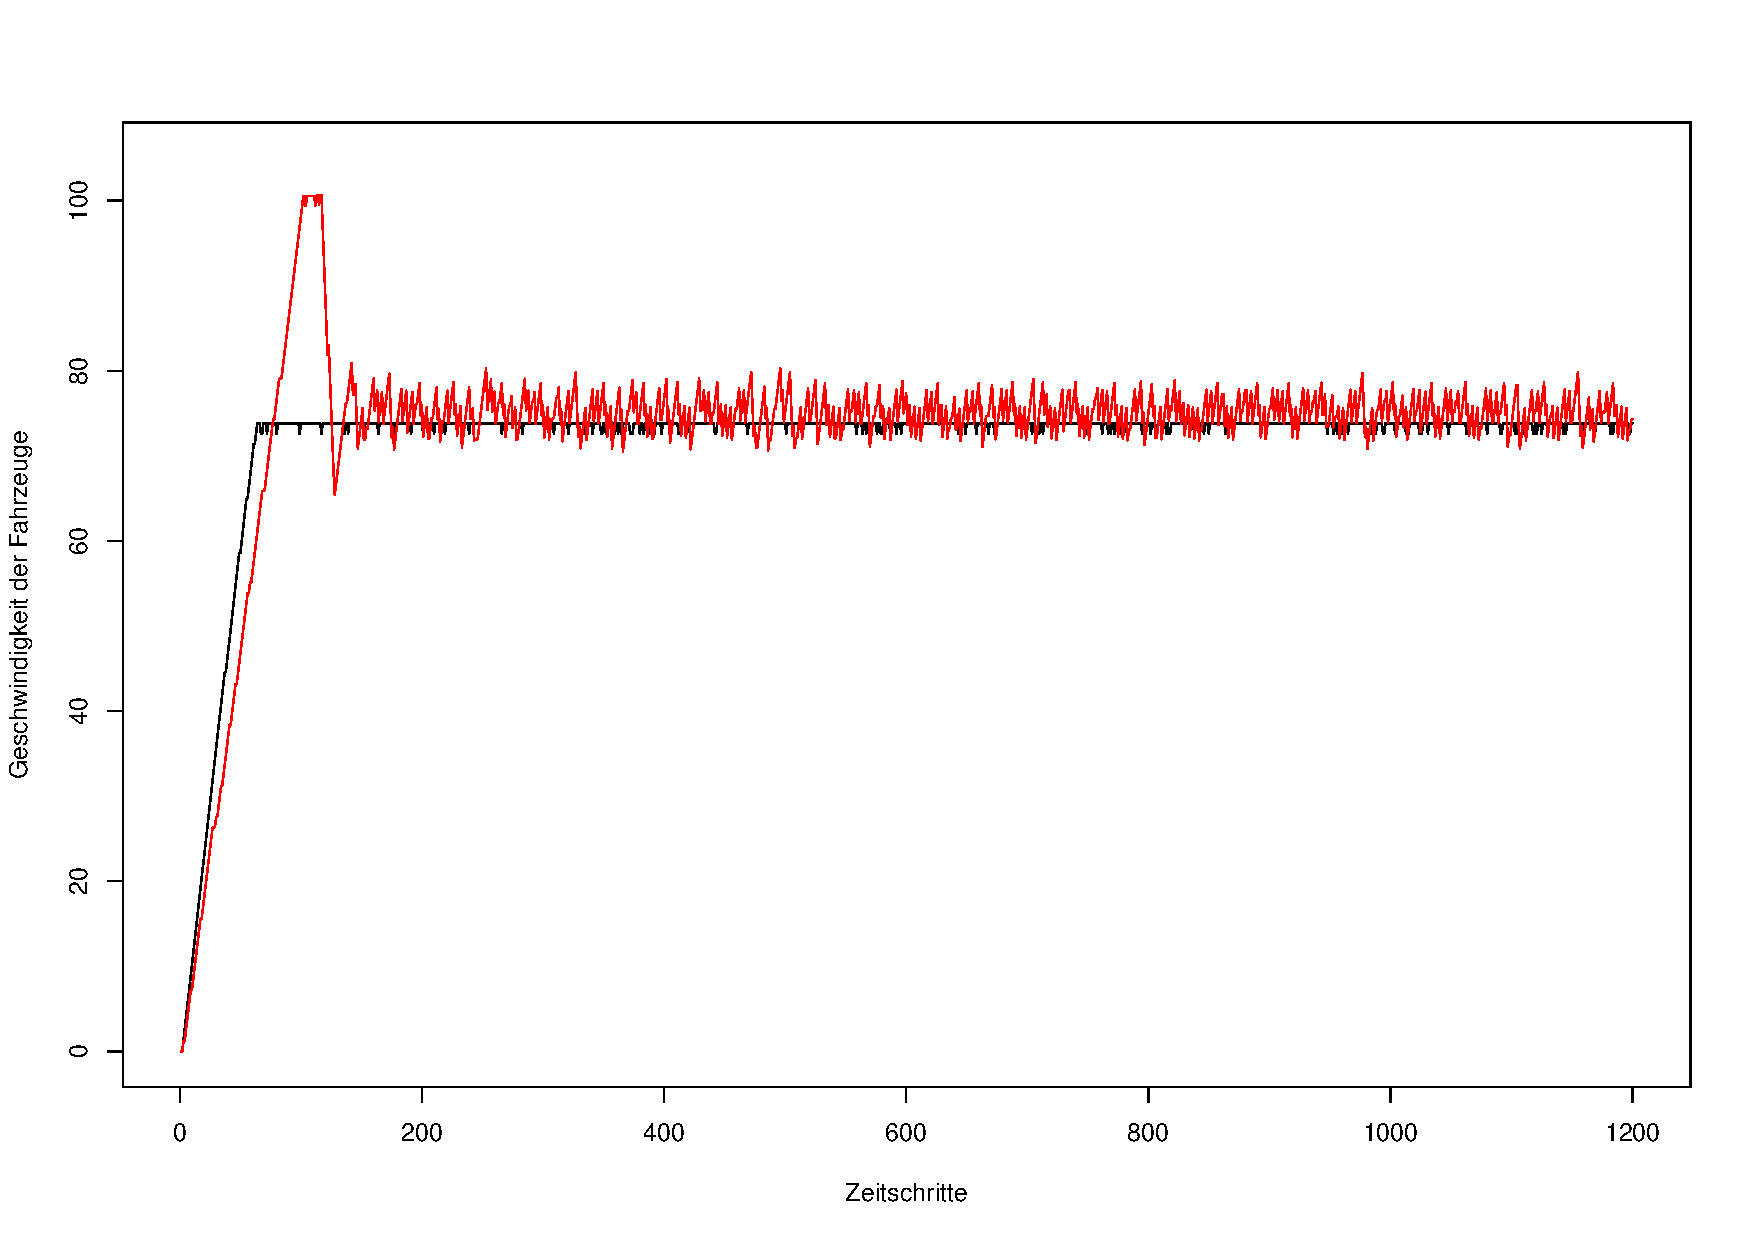
\includegraphics[width=0.9\textwidth]{speed_run27}
% \caption[kurzText]
% 		{Text}
% \label{figure:image1}
%\end{figure}
%
%
%\begin{figure}[hptb]
%  \centering 
%   \subfigure[Text1]{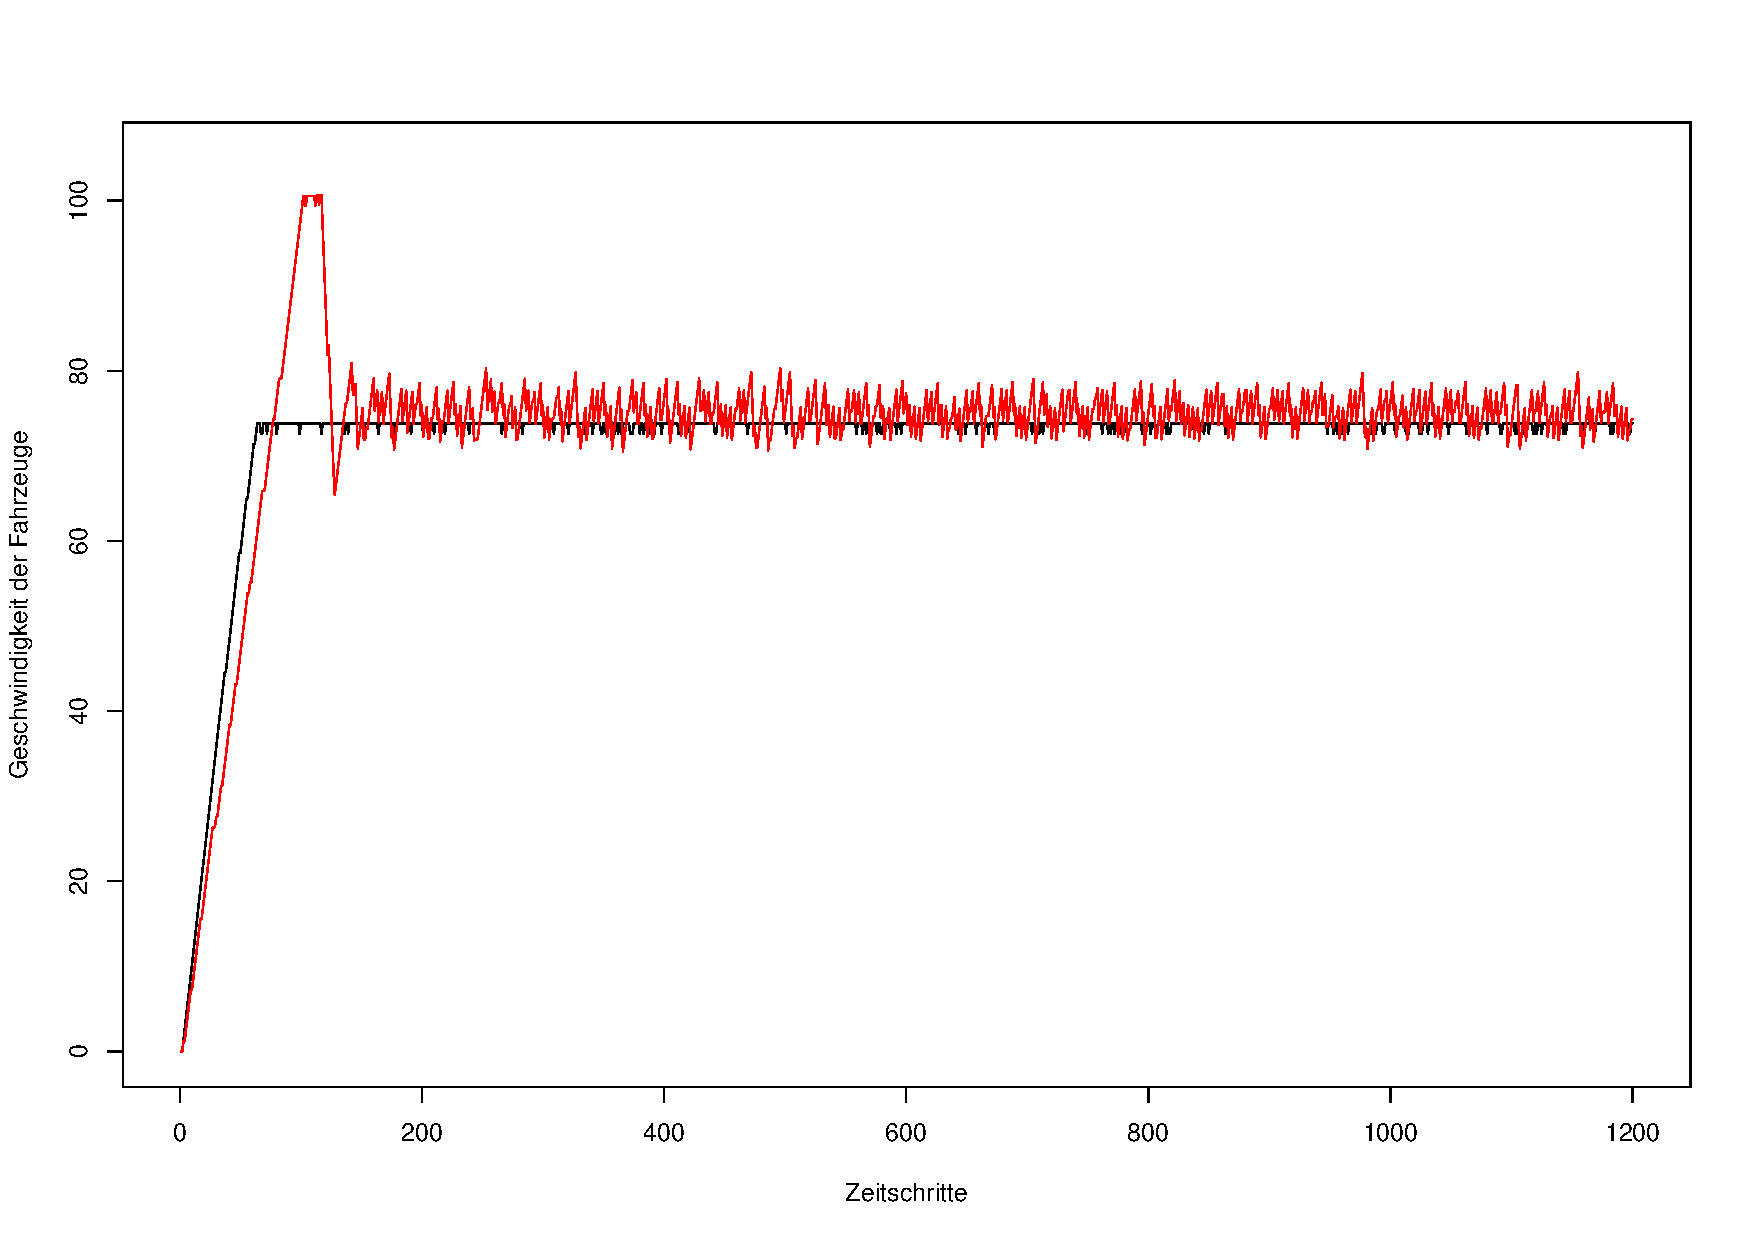
\includegraphics[width=0.45\textwidth]{speed_run27}\label{figure:image2-1}}\qquad 
%   \subfigure[Text2]{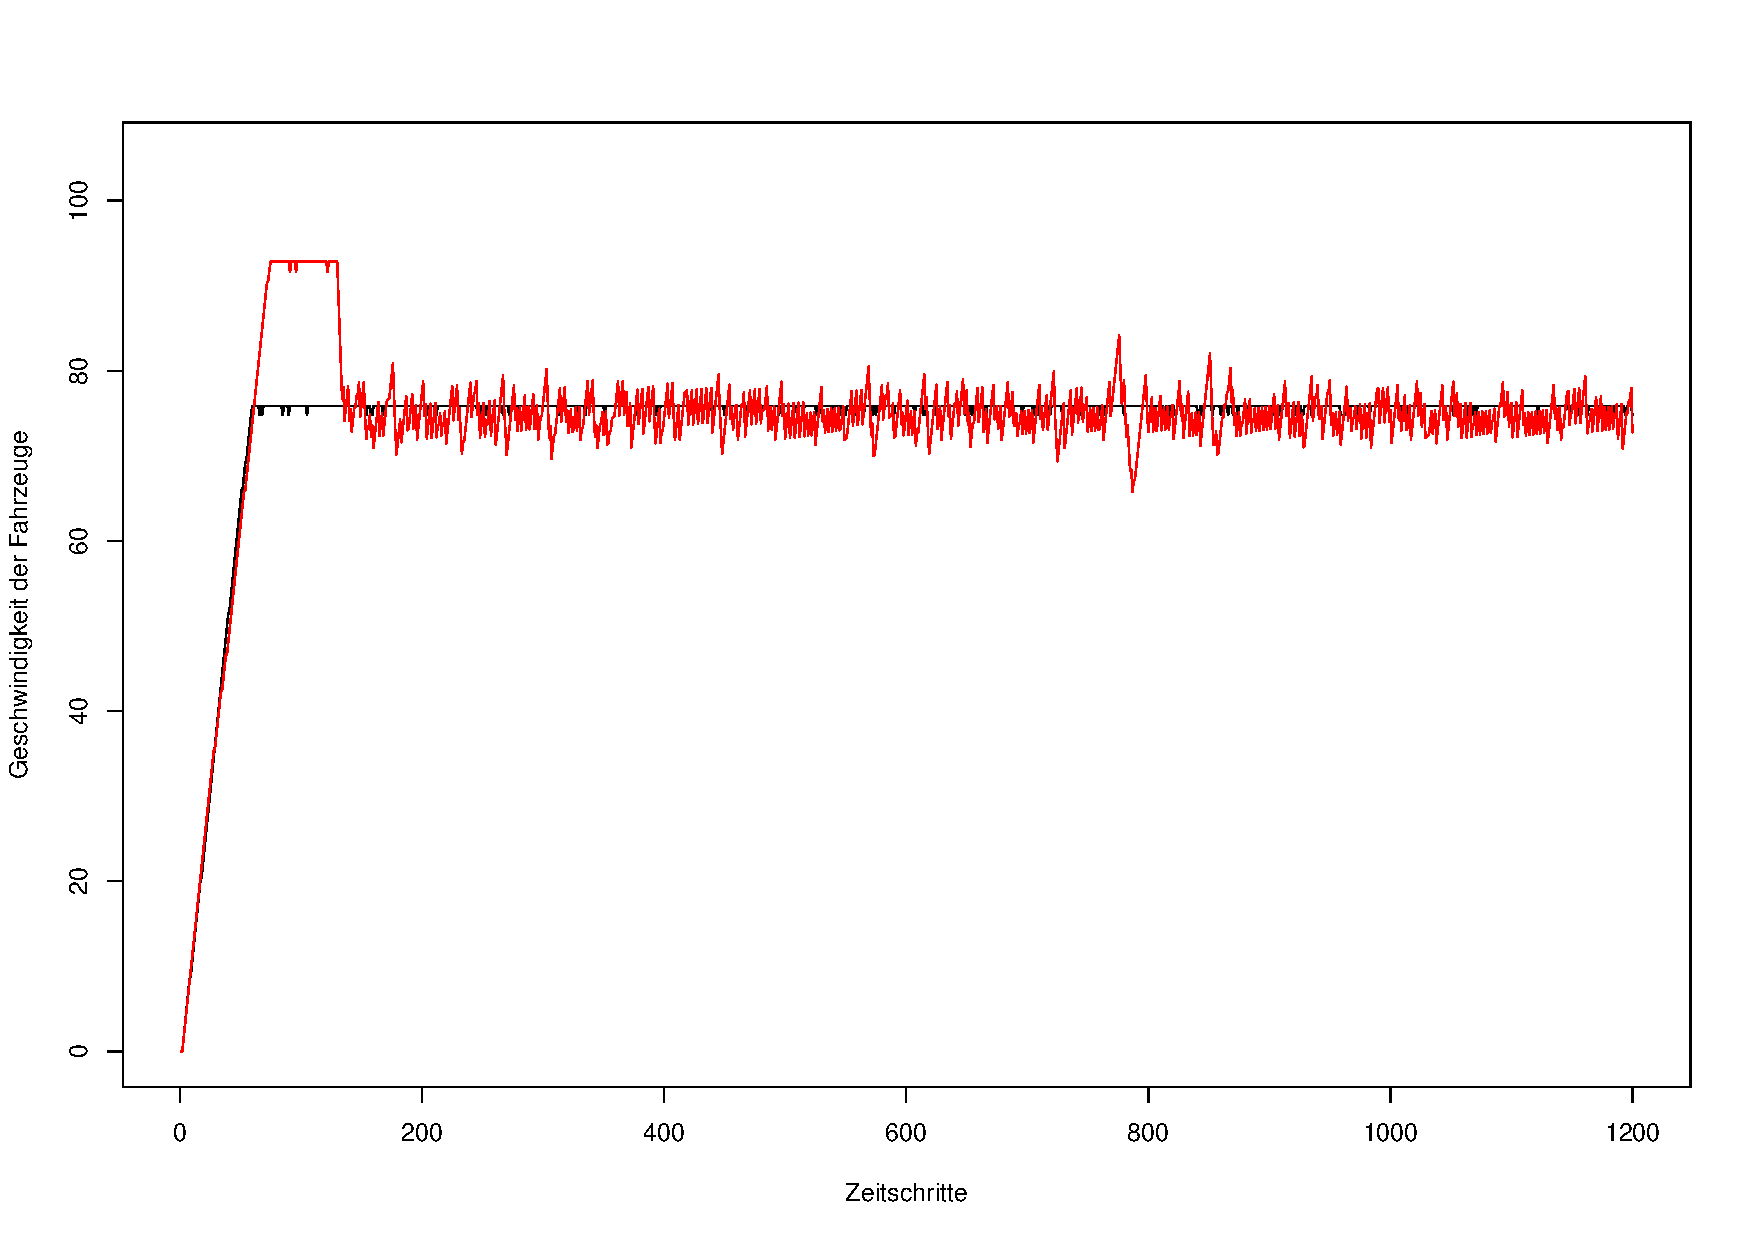
\includegraphics[width=0.45\textwidth]{speed_run28}\label{figure:image2-2}}  \caption{Text} 
%  \label{figure:image2}
%\end{figure}
%
%
%\begin{figure}[hptb]
%  \centering 
%   \subfigure[Text1]{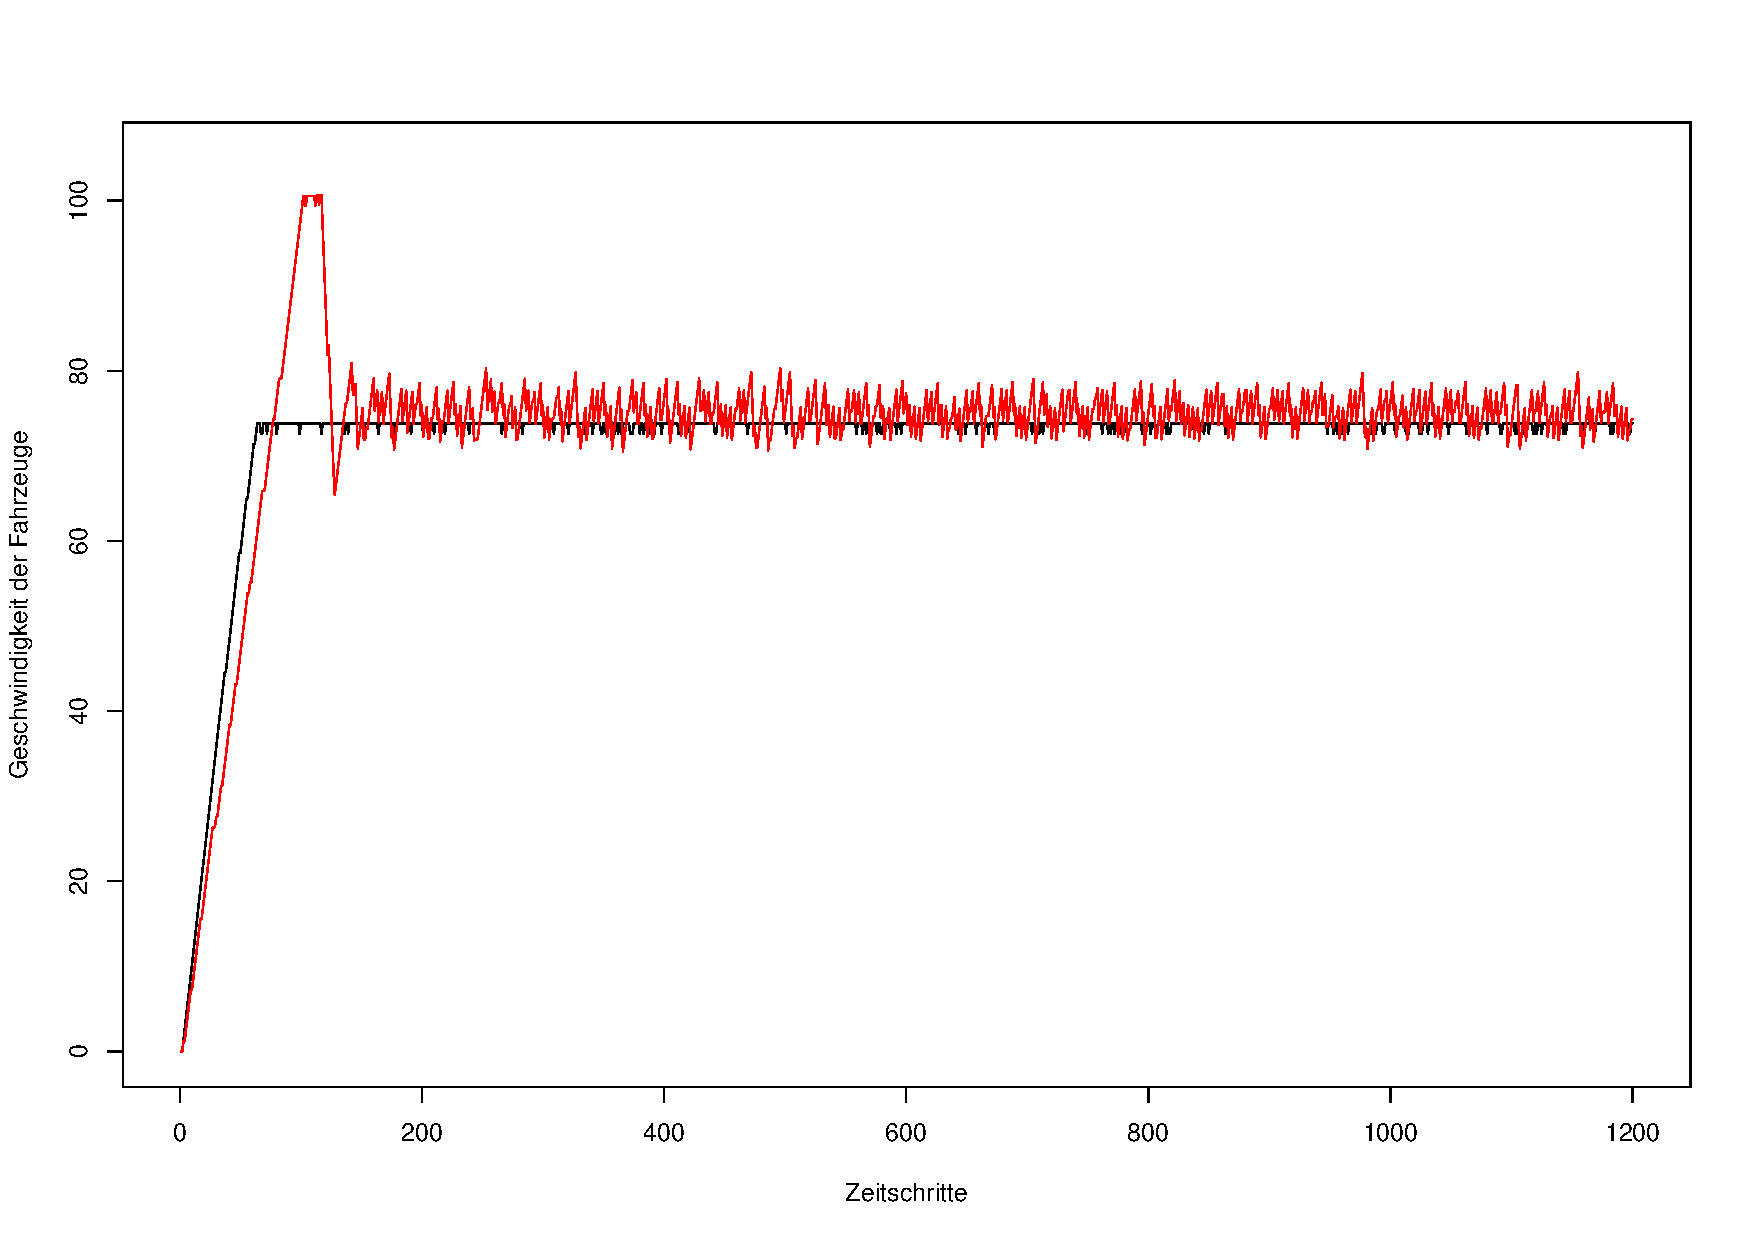
\includegraphics[width=0.3\textwidth]{speed_run27}\label{figure:image3-1}}\qquad 
%   \subfigure[Text2]{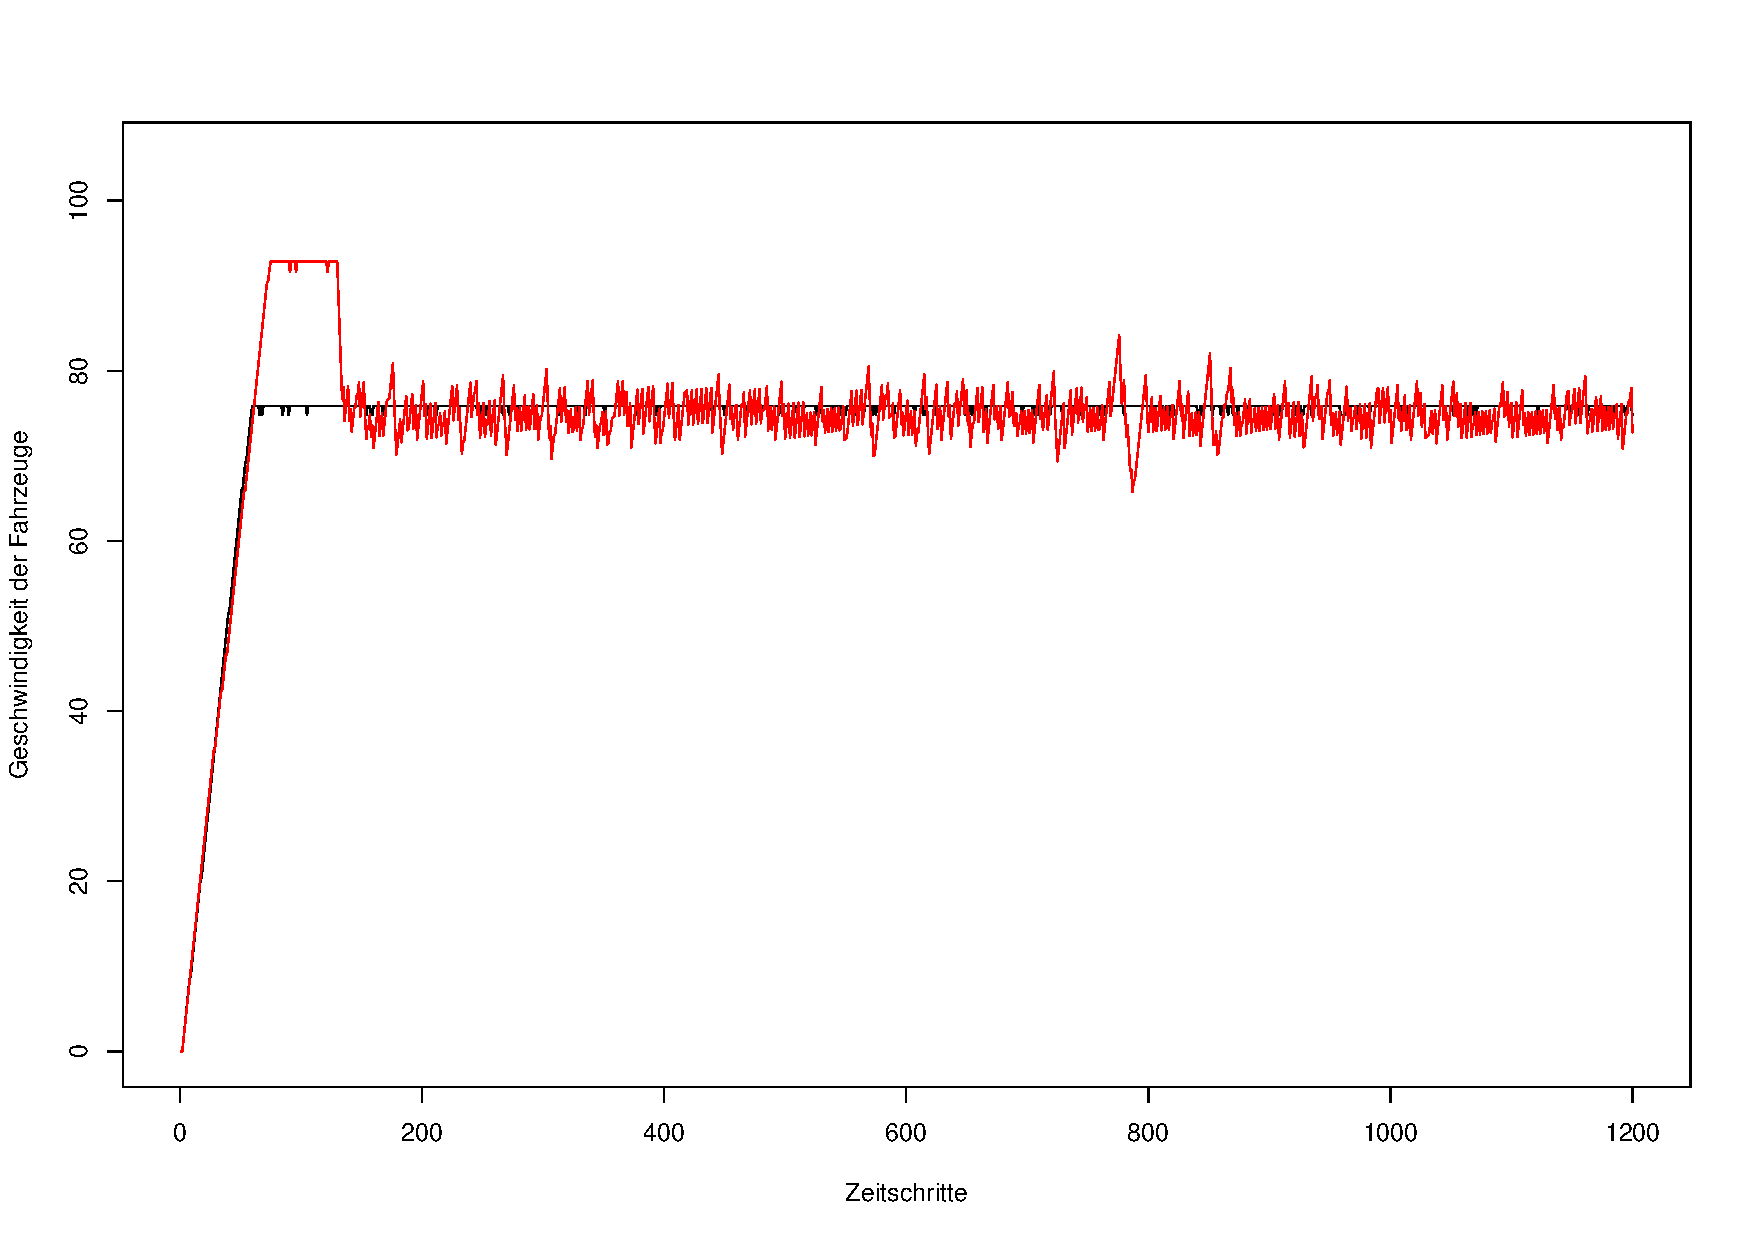
\includegraphics[width=0.3\textwidth]{speed_run28}\label{figure:image3-2}}\qquad 
%   \subfigure[Text3]{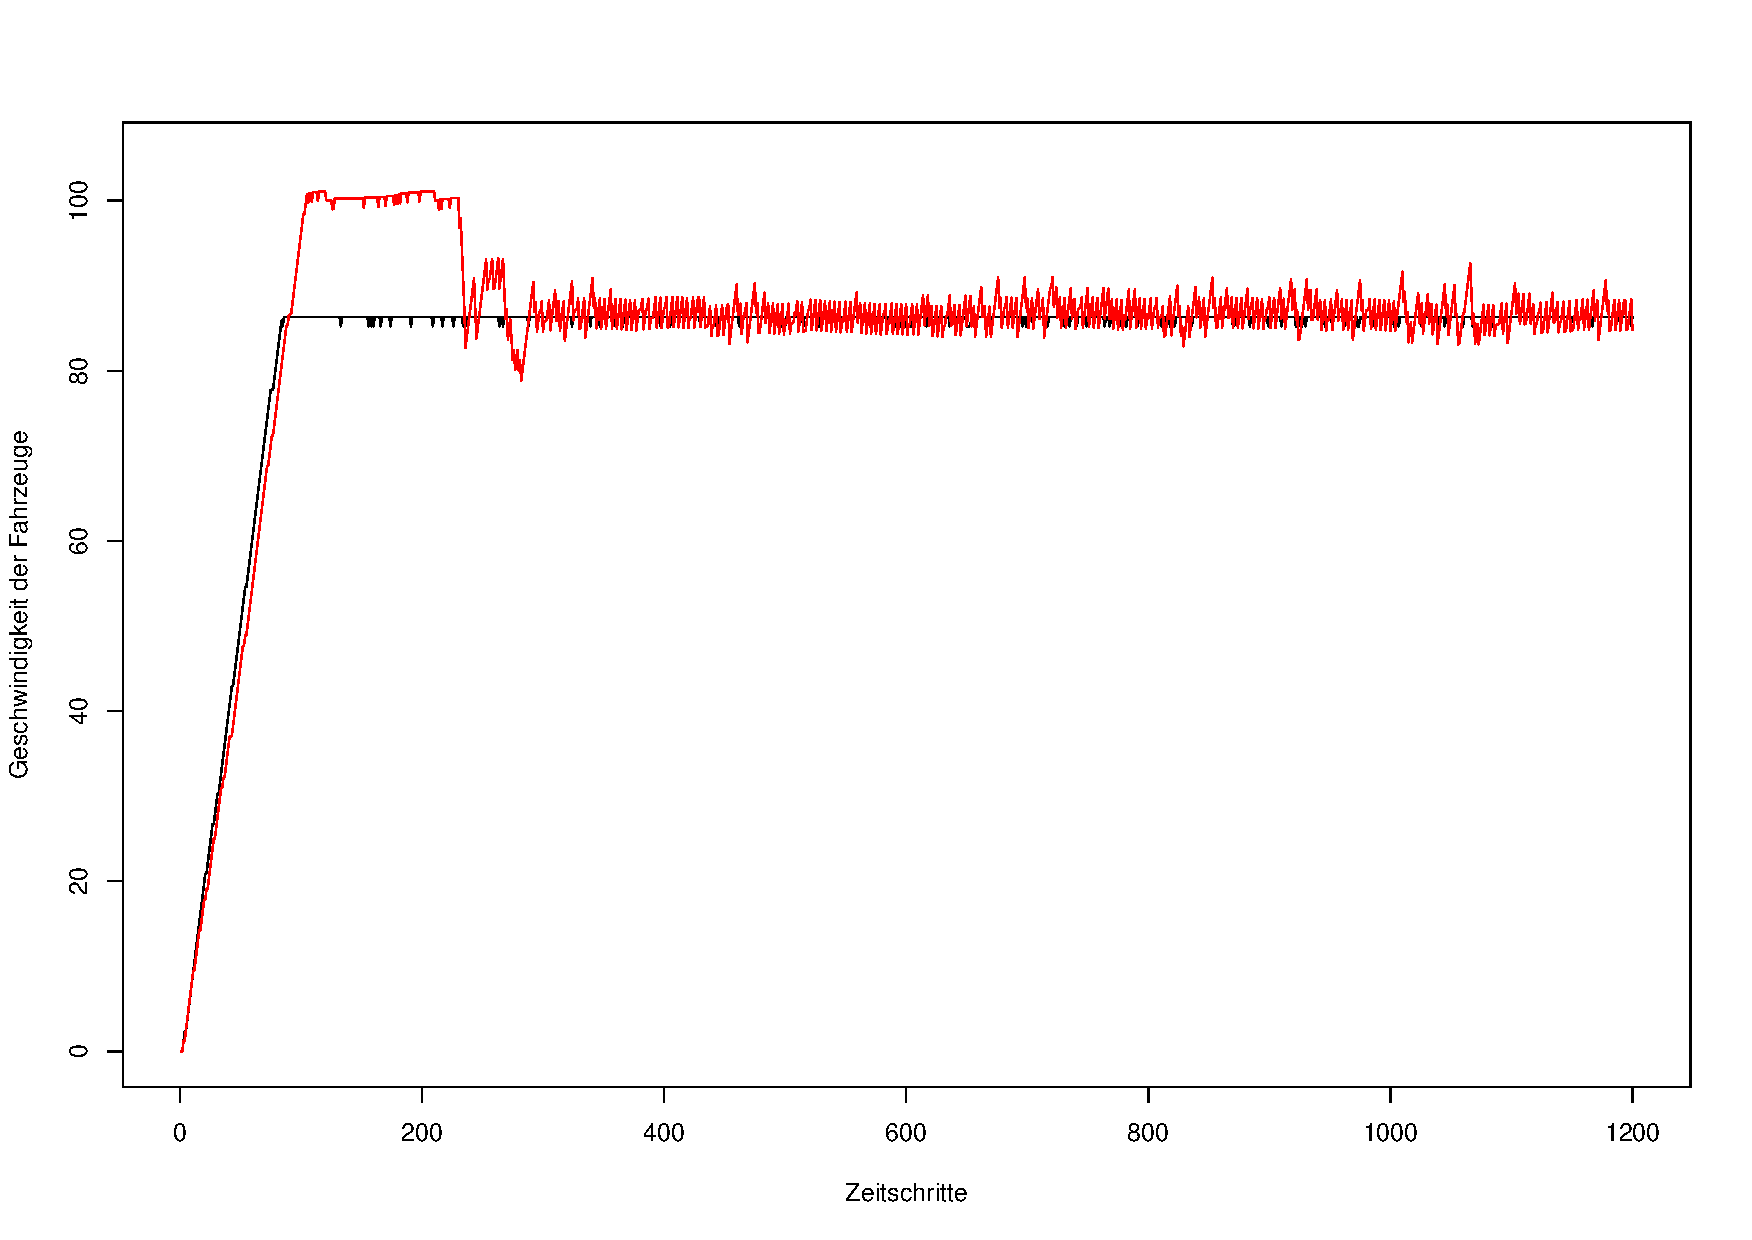
\includegraphics[width=0.3\textwidth]{speed_run29}\label{figure:image3-3}}
%  \caption{Text} 
%  \label{figure:image3}
%\end{figure}
%
